%杨舒云的实验报告编辑界面,使用了Huanyu Shi,2019级的模板,杨舒云在此拜谢ORZ!

%!TEX program = xelatex
\documentclass[dvipsnames, svgnames,a4paper,11pt]{article}
% ----------------------------------------------------- 
%	加边框的命令
%	参考:https://tex.stackexchange.com/questions/531559/how-to-add-the-page-border-for-first-two-pages-in-latex
\usepackage{tikz}
\usetikzlibrary{calc}
\usepackage{eso-pic}
\AddToShipoutPictureBG{%
\begin{tikzpicture}[overlay,remember picture]
\draw[line width=0.6pt] % 边框粗细
    ($ (current page.north west) + (0.6cm,-0.6cm) $)
    rectangle
    ($ (current page.south east) + (-0.6cm,0.6cm) $); % 边框位置
\end{tikzpicture}}


\usepackage{xcolor}
\definecolor{c1}{HTML}{086173} % 目录颜色 原版为2752C9 紫灰色535AAA 蓝紫色0B0DB7 深蓝色070F94 湖绿色219394 松石灰绿086173
\definecolor{c2}{HTML}{E20129} % 引用颜色 原版\definecolor{c2}{RGB}{190,20,83} 橙色F24729

\usepackage{ctex}
\usepackage[top=28mm,bottom=28mm,left=15mm,right=15mm]{geometry}
\usepackage{hyperref} 
\hypersetup{
	colorlinks,
	linktoc = section, % 超链接位置,选项有section, page, all
	linkcolor = c1, % linkcolor 目录颜色
	citecolor = c1  % citecolor 引用颜色
}
\usepackage{amsmath,enumerate,multirow,float}
\usepackage{tabularx}
\usepackage{tabu}
\usepackage{subfig}
\usepackage{fancyhdr}
\usepackage{graphicx}
\usepackage{wrapfig}  
\usepackage{physics}
\usepackage{appendix}
\usepackage{amsfonts}

%
\usepackage{tcolorbox}
\tcbuselibrary{skins,breakable}
\newtcolorbox{tbox}[2][]{
    colframe=black!70!,
    breakable,
    enhanced,
	boxrule =0.5pt,
    title = {#2},
    fonttitle = \large\kaishu\bfseries,
	drop fuzzy shadow,
    #1
}
\newtcolorbox[auto counter,number within=section]{question}[1][]{
  top=2pt,bottom=2pt,arc=1mm,
  boxrule=0.5pt,
%   frame hidden,
  breakable,
  enhanced, %跨页后不会显示下边框
  coltitle=c1!80!gray,
  colframe=c1,
  colback=c1!3!white,
  drop fuzzy shadow,
  title={思考题~\thetcbcounter:\quad},
  fonttitle=\bfseries,
  attach title to upper,
  #1
}

% ---------------------------------------------------------------------
%	利用cleveref改变引用格式,\cref是引用命令
\usepackage{cleveref}
\crefformat{figure}{#2{\textcolor{c2}{Figure #1}}#3} % 图片的引用格式
\crefformat{equation}{#2{(\textcolor{c2}{#1})}#3} % 公式的引用格式
\crefformat{table}{#2{\textcolor{c2}{Table #1}}#3} % 表格的引用格式


% ---------------------------------------------------------------------
%	页眉页脚设置
\fancypagestyle{plain}{\pagestyle{fancy}}
\pagestyle{fancy}
\lhead{\kaishu 中山大学物理与天文学院\uppercase\expandafter{\romannumeral1}} % 左边页眉,学院 + 课程
\rhead{\kaishu 杨舒云的实验报告} % 右边页眉,实验报告标题
\cfoot{\thepage} % 页脚,中间添加页码


% ---------------------------------------------------------------------
%	对目录、章节标题的设置
\renewcommand{\contentsname}{\centerline{\huge 目录}}
\usepackage{titlesec}
\usepackage{titletoc}
% \titleformat{章节}[形状]{格式}{标题序号}{序号与标题间距}{标题前命令}[标题后命令]
\titleformat{\section}{\centering\LARGE\songti}{}{1em}{}

% ---------------------------------------------------------------------
%   listing代码环境设置
\usepackage{listings}
\lstloadlanguages{python}
\lstdefinestyle{pythonstyle}{
backgroundcolor=\color{gray!5},
language=python,
frameround=tftt,
frame=shadowbox, 
keepspaces=true,
breaklines,
columns=spaceflexible,                   
basicstyle=\ttfamily\small, % 基本文本设置,字体为teletype,大小为scriptsize
keywordstyle=[1]\color{c1}\bfseries, 
keywordstyle=[2]\color{Red!70!black},   
stringstyle=\color{Purple},       
showstringspaces=false,
commentstyle=\ttfamily\scriptsize\color{green!40!black},%注释文本设置,字体为sf,大小为smaller
tabsize=2,
morekeywords={as},
morekeywords=[2]{np, plt, sp},
numbers=left, % 代码行数
numberstyle=\it\tiny\color{gray}, % 代码行数的数字字体设置
stepnumber=1,
rulesepcolor=\color{gray!30!white}
}




% ---------------------------------------------------------------------
%	其他设置
\def\degree{${}^{\circ}$} % 角度
\graphicspath{{./images/}} % 插入图片的相对路径
\allowdisplaybreaks[4]  %允许公式跨页 
\usepackage{lipsum}
\usepackage{adjustbox}
%\usepackage{mathrsfs} % 字体
\captionsetup[figure]{name=Figure} % 图片形式
\captionsetup[table]{name=Table} % 表格形式

\begin{document}
	
	
	
	% 实验报告封面	
	
	% 顶栏
	\begin{table}
		\renewcommand\arraystretch{1.7}
		\begin{tabularx}{\textwidth}{
				|X|X|X|X
				|X|X|X|X|}
			\hline
			\multicolumn{2}{|c|}{预习报告}&\multicolumn{2}{|c|}{实验记录}&\multicolumn{2}{|c|}{分析讨论}&\multicolumn{2}{|c|}{总成绩}\\
			\hline
			\LARGE25 & & \LARGE30 & & \LARGE25 & & \LARGE80 & \\
			\hline
		\end{tabularx}
	\end{table}
	% ---
	
	% 信息栏
	\begin{table}
		\renewcommand\arraystretch{1.7}
		\begin{tabularx}{\textwidth}{|X|X|X|X|}
			\hline
			年级、专业: & 2022级 物理学 &组号: & 2\\
			\hline
			姓名: & 杨舒云  & 学号: & 22344020\\
			\hline
			实验时间: & 2024/3/7 & 教师签名: & \\
			\hline
		\end{tabularx}
	\end{table}
	% ---
	
	% 大标题
	\begin{center}
		\LARGE Lab2-1 \quad 原子的发射和吸收光谱观测分析实验
	\end{center}
	% ---
	
	% 注意事项
	
	% 基本
	\textbf{【实验报告注意事项】}
	\begin{enumerate}
		\item 实验报告由三部分组成:
		\begin{enumerate}
			\item 预习报告:课前认真研读实验讲义,弄清实验原理;实验所需的仪器设备、用具及其使用、完成课前预习思考题;了解实验需要测量的物理量,并根据要求提前准备实验记录表格(可以参考实验报告模板,可以打印)。\textcolor{red}{\textbf{(20分)}}
			\item 实验记录:认真、客观记录实验条件、实验过程中的现象以及数据。实验记录请用珠笔或者钢笔书写并签名(\textcolor{red}{\textbf{用铅笔记录的被认为无效}})。\textcolor{red}{\textbf{保持原始记录,包括写错删除部分,如因误记需要修改记录,必须按规范修改。}}(不得输入电脑打印,但可扫描手记后打印扫描件);离开前请实验教师检查记录并签名。\textcolor{red}{\textbf{(30分)}}
			\item 数据处理及分析讨论:处理实验原始数据(学习仪器使用类型的实验除外),对数据的可靠性和合理性进行分析;按规范呈现数据和结果(图、表),包括数据、图表按顺序编号及其引用;分析物理现象(含回答实验思考题,写出问题思考过程,必要时按规范引用数据);最后得出结论。\textcolor{red}{\textbf{(30分)}}
		\end{enumerate}
		\textbf{实验报告就是将预习报告、实验记录、和数据处理与分析合起来,加上本页封面。\textcolor{red}{(80分)}}
		\item 每次完成实验后的一周内交\textbf{实验报告}(特殊情况不能超过两周)。
	\end{enumerate}
	
	% 安全
	\textbf{【实验安全注意事项】}	
	\begin{enumerate}
		\item 实验中光纤不能过度弯折;
		\item 信号强度不能过饱和值;
		\item 光源长时间通电后会发热,小心烫手,切换光源时务必注意(可等断电冷却后再碰);
		\item 请提前了解光纤光谱仪的基本工作原理与关键参数等。		
	\end{enumerate}
	
	% ---
	
	% 特别鸣谢
	\textbf{【特别鸣谢及模板说明】}	
	
	感谢2019级学长石寰宇为本实验报告提供\LaTeX 模板。\textcolor{red}{\textbf{由于原实验报告模板缺少实验编号,为方便在电脑上整理,故添加自命名编号Lab2-1}}
	% ---
	
	
	
	% 目录
	\clearpage
	\tableofcontents
	\clearpage
	% ---
	
	
	
	% 预习报告	
	
	% 小标题
	\setcounter{section}{0}
	\section{Lab2-1 原子的发射和吸收光谱观测分析实验 \quad\heiti 预习报告}
	% ---
	
	% 实验目的
	\subsection{实验目的}
	\begin{enumerate}
		\item CA3.1 原子发射光谱的观测
		\begin{enumerate}
			\item 学习光纤光谱仪的使用;
			\item 观测钠原子光谱,了解碱金属原子光谱的一般规律;
			\item 观测汞原子光谱,了解中外层电子与原子核相互作用;
			\item 观测多种光源的发射光谱,了解线光谱与连续谱的异同。
		\end{enumerate}
		
		\item CA3.2 原子吸收光谱的观测
		\begin{enumerate}
			\item 调配不同浓度的高锰酸钾水溶液;
			\item 测量高锰酸钾水溶液的紫外-可见吸收光谱,找出吸收峰;
			\item 测量不同浓度高锰酸钾水溶液的紫外-可见吸收光谱,验证比
			尔定律;
			\item 测量不同片数玻璃基板的透过光谱,验证朗伯定律。
		\end{enumerate}
	\end{enumerate}
	% ---
	
	% 仪器用具
	\subsection{仪器用具}
	\begin{table}[htbp]
		\centering
		\renewcommand\arraystretch{1.6}
		% \setlength{\tabcolsep}{10mm}
		\begin{tabular}{|p{0.05\textwidth}|p{0.20\textwidth}|p{0.05\textwidth}|p{0.5\textwidth}|}
			\hline
			编号& 仪器用具名称 & 数量 &  主要参数(型号,测量范围,测量精度等) \\
			\hline
			1& 多种光源 & 1 & 低压汞灯、低压钠灯、氢氘灯、 溴钨灯、多种颜色的发光二极管 \\
			\hline
			2& 滤光片 & 1 & 白片、红片 \\
			\hline
			3& 测控计算机 & 1 & -- \\
			\hline
			4& 光谱观测和分析仪器 & 1 & 光纤光谱仪 \\
			\hline
			5& 高锰酸钾水溶液 & -- & -- \\
			\hline
			6& 玻璃基板 & 1 & -- \\
			\hline
			7& 比色皿 & 1 & -- \\
			\hline
		\end{tabular}
	\end{table}
	% ---
	
	% 原理概述
	\subsection{原理概述}
	
	\subsubsection{CA3.1 原子发射光谱的观测}
	\begin{enumerate}
		\item 碱金属原子光谱
		\begin{enumerate}
			\item 碱金属原子具有相对简单的电子结构,其原子核外只有一个价电子。这个外层电子非常容易被激发到更高的能级,当它返回到低能级时,会发射特定波长的光。这使得碱金属原子的光谱特性与内层电子的结构密切相关。例如,钠原子具有11个电子,其中10个为内层电子,1个为价电子。
			
			\begin{figure}[htbp]
				\centering
				\includegraphics[width=0.5\textwidth]{Lab2_1Gra1.jpg}
				\caption{碱金属原子光谱(图片来源于网络)}
				\label{fig:fig1}
			\end{figure}
			
			\item 碱金属原子光谱中,谱线的波数($\bar{\nu}$)可以通过里德伯公式来表示:
			\[
			\tilde{\nu} = R \left( \frac{1}{n_1^{*2}} - \frac{1}{n_2^{*2}} \right)=\dfrac{R}{(n'-\mu'_{l'})^2}-\dfrac{R}{(n-\mu_{l})^2}
			\]
			其中,$R$是里德伯常数,$n_1^*$和$n_2^*$分别是初始和最终能级的有效量子数。l与l'分别为该量子数决定之能级的轨道量子数;
			$\mu_{l}$与$\mu'_{l'}$分别为始态和终态的量子缺(也称量子改正数,量子亏损)。
			\item 钠原子的光谱中存在四个主要的线系:主线系、尖线系、漫线系和基线系,每个线系对应于不同能级跃迁的光谱线。具体到某一线系,例如主线系,其谱线的波数可以具体表示为上述里德伯公式的特定情况。
			
			对于某一线系谱线的波数公式可写为:
			\[\tilde{\nu} = A_{n'l'}-\dfrac{R}{(n-\mu_{l})^2}\]
			
			所有线系的共同特点包括,随着能级跃迁的增加,谱线趋于密集并向较短的波长方向(紫外区)收敛。同一线系内,愈向短波方向,相邻谱线的波数差愈小,最后趋于一个极限——连续谱与分立谱的边界。这是由于能量愈高,能级愈密,最后趋于连续。在同一线系内,愈向短波方向,谱线强度愈小,原因是能级愈高,将原子从基态激发到那一状态也愈不容易。
			
			不同线系的区别主要在于它们所涉及的能级跃迁不同,导致它们出现在光谱的不同区域,例如,某些线系可能在可见光区域,而其他线系则可能在紫外或红外区域。
			在光谱学中,称主线系的第一组线(双线)为共振线,钠原子的共 振线就是有名的黄双线(589.0nm 和 589.6nm)。
			从谱线的外表上看,主线系强度较大,锐线系轮廓清晰,漫 线系显得弥漫,一般复双重线连成一片。
		\end{enumerate}
		
		\item 单色仪色散系统:单色仪通过使用色散元件(如棱镜或衍射光栅)将入射光分离成其组成的单色光。色散系统的选择(棱镜或光栅)以及其配置(如光栅的线密度)直接影响到光谱仪的分辨率和可测量的波长范围。
		
		\begin{figure}[htbp]
			\centering
			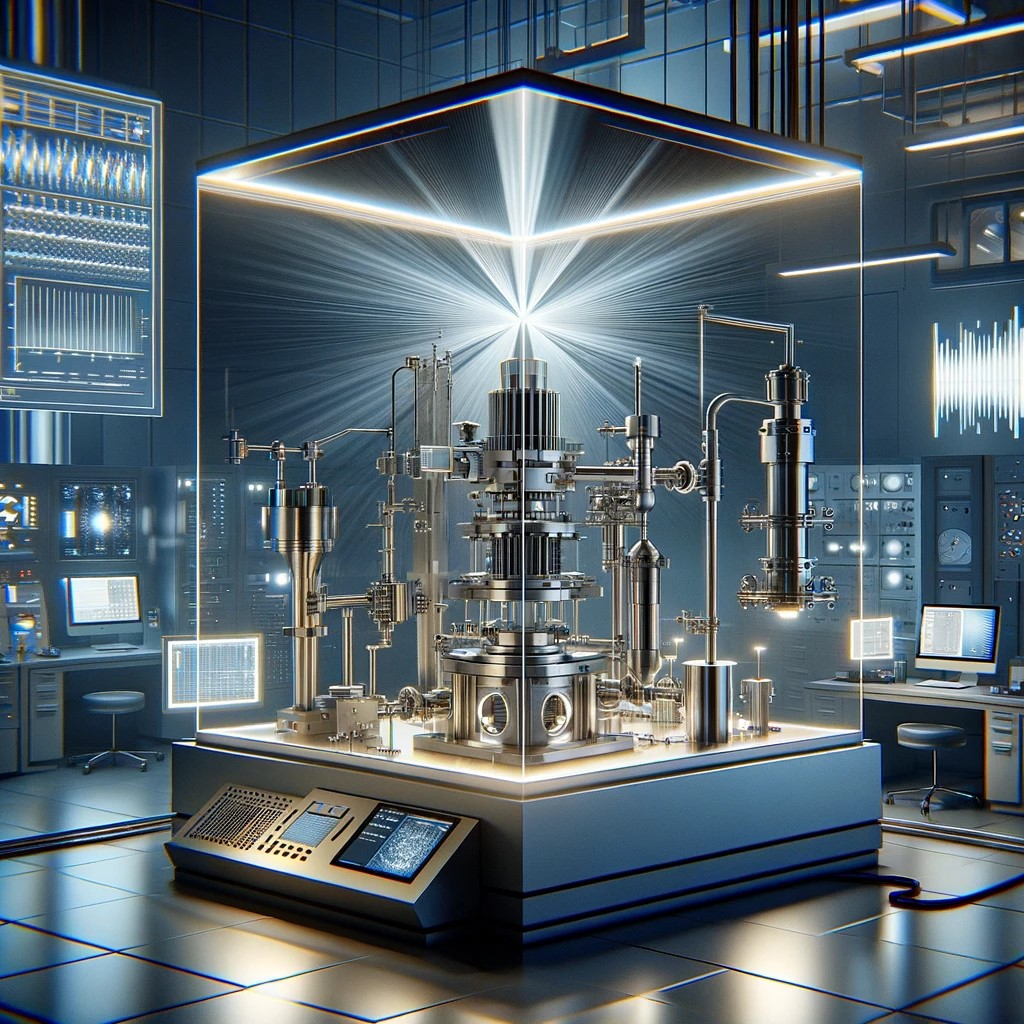
\includegraphics[width=0.4\textwidth]{Lab2_1Gra2.jpg}
			\caption{单色仪色散系统}
			\label{fig:fig2}
		\end{figure}
		
		\item 光谱仪和光学多通道分析仪:光谱仪利用光学元件收集来自样品的发射或吸收光,并通过色散系统对这些光进行分析,从而获得样品的光谱特性。光学多通道分析仪(OMA)是一种高性能的光谱仪,它可以同时收集多个波长的数据,大大提高了数据采集的效率和精度。OMA系统通常包括单色仪、光电探测器(如CCD或CMOS传感器)、以及用于数据处理的计算机系统。
	\end{enumerate}
	
	\subsubsection{CA3.2 原子吸收光谱的观测}
	\begin{enumerate}
		\item 光的吸收
		\begin{enumerate}
			\item 原子和分子吸收光的原理基于量子力学。当原子或分子吸收一定能量的光子时,会从一个能级跃迁到更高的能级。这个过程称为激发态,激发态的原子或分子可以通过辐射或非辐射过程返回到基态,其中辐射过程会发射光子。
			\item Planck公式描述了光子的能量与其频率的关系:
			\[ E = h\nu \]
			其中,\(E\) 是光子的能量,\(h\) 是Planck常数(\(6.62607015 \times 10^{-34}\) J·s),\(\nu\) 是光的频率。
			\item 光的吸收是指当物质(如原子、分子)接收到光能时,使得电子从较低的能级跃迁到较高的能级的过程。这一过程导致特定波长的光减弱,表现为吸收光谱。光的吸收也是指光经过物质时,部分光能被物质吸收,导致通过物质的光强度减弱的现象。这一过程与物质中的原子、分子能级结构有关,只有当光子能量与原子或分子能级差相匹配时,吸收才会发生。
			
			不同波长的光被吸收的特性取决于物质的电子结构(不同波长的光被吸收的特性取决于原子或分子能级结构的差异)。不同原子或分子根据其能级差异,会吸收不同波长(或频率)的光。每种原子或分子只吸收特定波长(即能量)的光,这些特定的波长对应于原子或分子内部能级之间的能量差。这种特性使得吸收光谱能够作为识别和分析化学物质的重要工具。因此,通过分析样品对不同波长光的吸收特性,可以得知样品中含有哪些元素。
		\end{enumerate}
		
		\item Lambert定律
		\begin{enumerate}
			\item Lambert定律描述了描述了无色散介质中光强度随穿过物质厚度的指数衰减规律,表明光的吸收与通过介质的路径长度成正比。
			
			\begin{figure}[htbp]
				\centering
				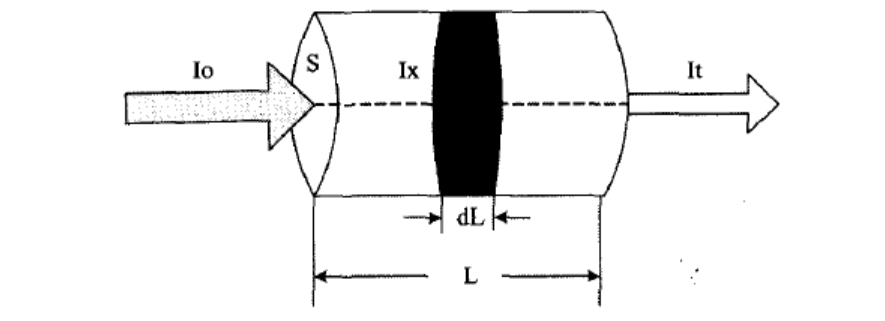
\includegraphics[width=0.45\textwidth]{Lab2_1Gra3.png}
				\caption{Lambert定律}
				\label{fig:fig3}
			\end{figure}
			
			\item Lambert定律的数学表达式为:
			\[ I = I_0 e^{-\alpha l} \]
			其中,\(I\) 是经过物质后的光强,\(I_0\) 是初始光强,\(\alpha\) 是吸收系数,\(l\) 是光通过物质的长度。
		\end{enumerate}
		
		\item Beer定律
		\begin{enumerate}
			\item Beer定律描述了溶液的浓度与它吸收特定波长光的能力之间的关系,表明吸收强度与溶质的浓度成正比。
			
			\begin{figure}[htbp]
				\centering
				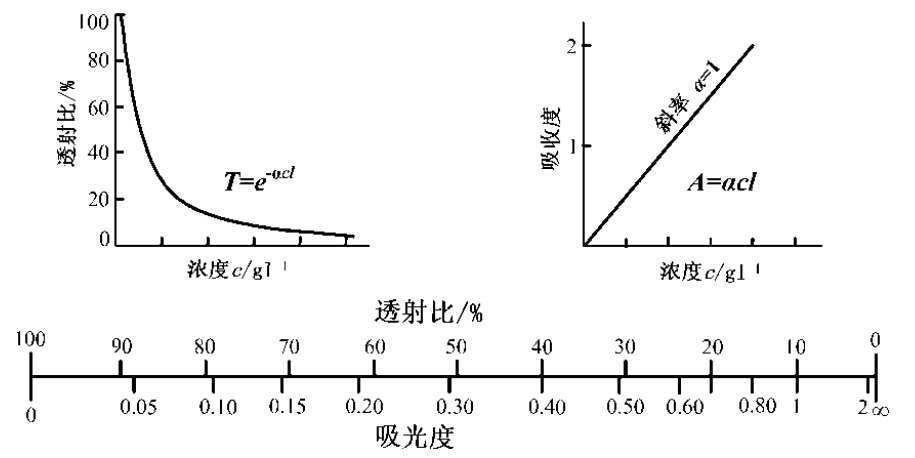
\includegraphics[width=0.6\textwidth]{Lab2_1Gra4.png}
				\caption{Beer定律}
				\label{fig:fig4}
			\end{figure}
			
			\item Beer定律的数学表达式为:
			\[ A = \epsilon c l \]
			其中,\(A\) 是吸光度,\(\epsilon\) 是摩尔吸光系数,\(c\) 是溶质的浓度,\(l\) 是光通过溶液的路径长度。
		\end{enumerate}
		
		\item 结合Lambert定律和Beer定律,我们得到Lambert-Beer定律:
		\[ A = \epsilon c l = \log \frac{I_0}{I} \]
		这表明吸光度与经过介质后的光强比的对数成正比,是分析化学中定量分析物质浓度的基础公式。
		
		\begin{figure}[htbp]
			\centering
			\subfloat[]{
				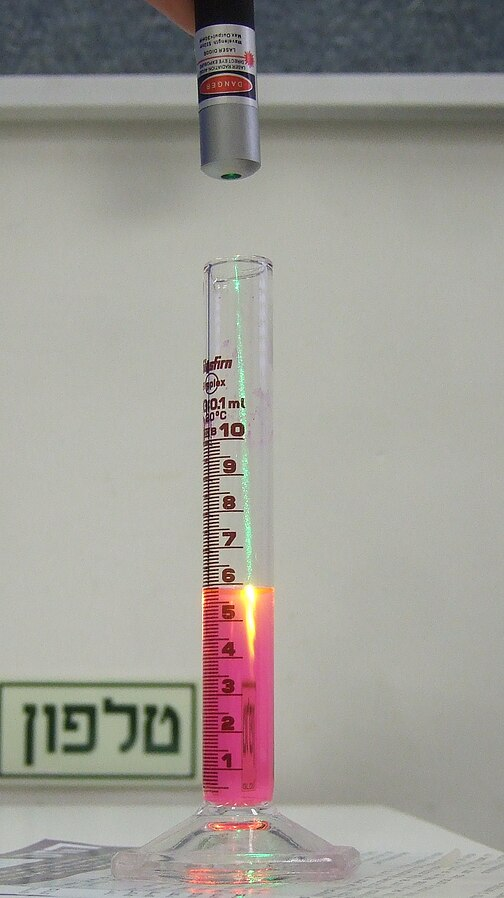
\includegraphics[width=0.2\textwidth]{Lab2_1Gra5.jpg}
			}
			\subfloat[]{
				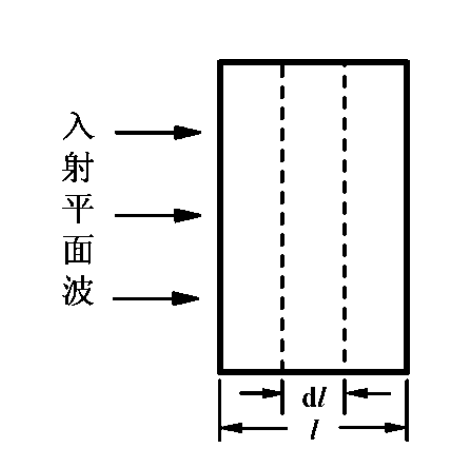
\includegraphics[width=0.4\textwidth]{Lab2_1Gra6.png}
			}
			\caption{Lambert-Beer定律}
			\label{fig:fig5}			
		\end{figure}
		
	\end{enumerate}
	% ---
	
	
	
	% 实验前思考题
	\subsection{实验前思考题}
	
	% 思考题1
	\begin{question}
		日常生活中,光源可以分为热光源和冷光源,请分别说明太阳光、蜡烛、白炽灯、荧光灯、 LED 灯等属于哪一类光源,为什么?
	\end{question}
	在日常生活中,光源可以分为热光源和冷光源两大类。这一分类基于光源发光的物理原理和其发出光的特性。以下是对几种光源的归类及其原因的解释:
	
	\begin{enumerate}
		\item 太阳光:太阳光是一种自然的热光源。它来自太阳的热辐射,太阳表面的高温使得其能够发出光线和热量。
		\item 蜡烛:蜡烛属于热光源。当蜡烛燃烧时,其产生的热量使得蜡烛的燃料发光,产生光线。
		\item 白炽灯:白炽灯是热光源的一种。它通过电流加热灯丝(通常是钨丝),使其达到高温并发光。这种光源的特点是大部分能量以热量的形式散失。
		\item 荧光灯:荧光灯属于冷光源。它使用电流激发气体或汞蒸气产生紫外光,紫外光随后激发涂在灯管内壁的荧光粉发出可见光。相比于白炽灯,荧光灯的热量释放较少,效率更高。
		\item LED灯:LED灯是冷光源。它通过半导体材料在电流作用下直接产生光,其转换效率高,发热量低,因此被认为是冷光源。
	\end{enumerate}
	
	总结如下,太阳光、蜡烛和白炽灯属于热光源,因为它们的光主要通过物质加热发出;而荧光灯和LED灯则是冷光源,这是因为它们通过电子激发而非加热产生光。每种光源的特点和应用场景不同,选择合适的光源可以根据具体需求和能效来决定。
	
	
	% ---
	
	
	
	% 实验记录	
	\clearpage
	
	% 顶栏
	\begin{table}
		\renewcommand\arraystretch{1.7}
		\centering
		\begin{tabularx}{\textwidth}{|X|X|X|X|}
			\hline
			专业: & 物理学 & 年级: & 2022级 \\
			\hline
			姓名: & 杨舒云 & 学号: & 22344020\\
			\hline
			室温: &  & 实验地点: &  \\
			\hline
			学生签名:& 杨舒云 & 评分: &\\
			\hline
			实验时间:& 2024// & 教师签名:&\\
			\hline
		\end{tabularx}
	\end{table}
	% ---
	
	% 小标题
	\section{Lab2-1 原子的发射和吸收光谱观测分析实验  \quad\heiti 实验记录}
	% ---
	
	% 实验过程记录
	\subsection{实验内容、步骤与结果}
	
	%
	\subsubsection{操作步骤记录}
	\begin{enumerate}
		\item \textbf{CA3.1 原子发射光谱的观测}实验操作步骤:
		\begin{enumerate}
			\item 正确连接光谱仪和光源。
			\item 打开软件,确认光谱仪连接正确。
			\item 打开光源,开始测量,自动设置积分时间,再手动调整积分时间和平均次数。
			\item 调整信号强度至饱和值的80%左右。
			\item 分别测量钠灯、汞灯的光谱,并保存光谱图片和实验数据。
			\item 观测记录实验室电灯(改为手机闪光灯)、手机屏光谱,分析光谱特点。
		\end{enumerate}
				
		\item \textbf{CA3.2 原子吸收光谱的观测}实验操作步骤:
		\begin{enumerate}
			\item 准备不同浓度的高锰酸钾溶液。
			\item 正确链接光谱仪和光源,放置纯水样品进行测试。
			\item 打开软件,确认光谱仪连接正确。
			\item 打开光源,开始测量,自动设置积分时间,再手动调整。
			\item 存储参考背景和暗背景。
			\item 更换样品,测量吸收光谱。
			\item 选择吸光度模式,实时显示测量结果,并保存数据。
			\item 对比之前保存的实验数据。
			\item 验证比尔定律,测量记录各种浓度的高锰酸钾溶液吸收曲线,并找出吸收峰波长。
			\item 验证朗伯定律,记录不同片数玻璃基板的透过光谱曲线,分析透过率与玻璃基板厚度的关系。
		\end{enumerate}
	\end{enumerate}	
	
	%
	\subsubsection{实验数据记录}
	\begin{enumerate}
		\item 钠灯光谱
		\item 汞灯光谱
		\item 手机屏光谱
		\item 手机闪光灯光谱
		\item Beer定律验证
		\item Lambert定律验证
	\end{enumerate}
	
	% ---
	
	% 原始数据
	\clearpage
	\subsection{原始数据记录}
	实验记录本上的原始数据见%\cref{}(签字)。
	
	实验台桌面整理见%\textbf{附件}部分(\cref{})。
	
	其它原始数据见%\cref{}。
	% ---
	
	% 问题记录
	\subsection{实验过程中遇到的问题记录}
	\begin{enumerate}
		\item 
	\end{enumerate}
	% ---
	
	
	
	% 分析与讨论	
	\clearpage
	
	% 顶栏
	\begin{table}
		\renewcommand\arraystretch{1.7}
		\begin{tabularx}{\textwidth}{|X|X|X|X|}
			\hline
			专业:& 物理学 &年级:& 2022级\\
			\hline
			姓名: & 杨舒云 & 学号:& 22344020\\
			\hline
			日期:& 2023/11/23 & 评分: &\\
			\hline
		\end{tabularx}
	\end{table}
	% ---
	
	% 小标题
	\section{Lab2-1 原子的发射和吸收光谱观测分析实验 \quad\heiti 分析与讨论}
	% ---
	
	% 数据处理
	\subsection{实验数据分析}
	
	%
	\subsubsection{钠灯光谱、汞灯光谱的谱线分析}
	\begin{enumerate}
		\item 
	\end{enumerate}
	
	%
	\subsubsection{电灯(手机闪光灯)、手机屏幕光谱分析}
	\begin{enumerate}
		\item 
	\end{enumerate}
	
	%
	\subsubsection{Beer定律验证}
	
	%
	\subsubsection{Lambert定律验证}
	
	% ---
	
	% 实验后思考题
	\subsection{实验后思考题}
	
	%思考题1
	\begin{question}
		
	\end{question}
	
	% 思考题2
	\begin{question}
		
	\end{question}
	
	% 思考题3
	\begin{question}
		
	\end{question}
	
	% ---
	
	
	% 结语部分
	\clearpage
	
	% 小标题
	\section{Lab2-1 原子的发射和吸收光谱观测分析实验 \quad\heiti 结语}
	% ---
	
	% 总结、杂谈与致谢
	\subsection{总结、杂谈与致谢}
	\begin{enumerate}
		\item 
	\end{enumerate}
	% ---
	
	% 参考文献
	\subsection{参考文献}
	[1] 维基百科 https://zh.wikipedia.org
	
	[2] 沈韩.基础物理实验.——北京:科学出版社,2015.2 ISBN:978-7-03-043311-4
	
	% ---
	
	% 附件
	\subsection{附件}
	试验台桌面整理如%\cref{}所示。
	
	实验报告个人签名如\cref{fig:name}。
	
	\begin{figure}[htbp]
		\centering
		
\includegraphics[width=0.7\textwidth]{name.png}
		\caption{个人签名}
		\label{fig:name}
	\end{figure}
	
	% ---
	
	相关代码已上传至Github。
	
	
	
\end{document}